\section{Inne ważne elementy Win32API}

\subsection{Biblioteki ładowane dynamicznie}

Oprócz statycznego łączenia bibliotek podczas linkowania programu, w Windows istnieje możliwość 
ładowania kodu w trakcie działania aplikacji. Wiele z dotyczchczas wykorzystywanych funkcji znajduje się
w takich właśnie modułach: KERNEL32.DLL, GDI32.DLL, czy USER32.DLL. Tworzenie bibliotek funkcji zasadne jest tam,
gdzie pewna funkcjonalność może być współdzielona przez wiele różnych modułów. Zastosowanie bibliotek
oznacza zmieniejszenie zapotrzebowania pamięci, ponieważ system potrafi zoptymalizować przydział pamięci
dla biblioteki dołączanej dynamicznie.


Przykład biblioteki:

\begin{scriptsize}
\begin{verbatim}
/* Wiktor Zychla 2003 */
#include <windows.h>

#ifdef __cplusplus
#define EXPORT extern "C" __declspec (dllexport)
#else
#define EXPORT __declspec (dllexport)
#endif

EXPORT int MojaFunkcja();

BOOL WINAPI DllMain(HINSTANCE hinstDLL, DWORD fwdreason, LPVOID lpvReserved)
{
        return 1;
}

int MojaFunkcja()
{
        return 1;
}
\end{verbatim}
\end{scriptsize}

Program, który korzysta z biblioteki:

\begin{scriptsize}
\begin{verbatim}
/* Wiktor Zychla 2003 */
#include <windows.h>
#include <stdio.h>

const char libName[] = "abcLib.dll";

int main()
{
    typedef int(*pfPInt)();
    pfPInt  myFunc;

    HMODULE hLibrary;
    
    hLibrary = LoadLibrary(libName);

    if (hLibrary == NULL) 
    {
       MessageBox(NULL, "Blad ladowania biblioteki", "", MB_OK);
       return 1;
    }
    
    myFunc = (pfPInt)GetProcAddress(hLibrary, "MojaFunkcja");
    
    if (myFunc == NULL)
    {
       MessageBox(NULL, "Blad ladowania funkcji", "", MB_OK);
       return 1;
    }
    
    char buf[80];

    int res = myFunc();
	sprintf( buf, "Wynik : %d", res );
    MessageBox(NULL, buf, "", MB_OK);
    
    FreeLibrary(hLibrary);

    return 0;
      
}
\end{verbatim}
\end{scriptsize}

\subsection{Różne przydatne funkcje Win32API}

\begin{itemize}

\item Typowe okno informacyjne tworzy się za pomocą funkcji
\begin{scriptsize}
\begin{verbatim}
int MessageBox(

    HWND hWnd,          // uchwyt okna-właściciela
    LPCTSTR lpText,     // treść komunikatu
    LPCTSTR lpCaption,  // treść opisu komunikatu
    UINT uType          // styl komunikatu (dodatkowe ikony, przyciski)
   );
\end{verbatim}
\end{scriptsize}

\item Tekst pokazywany na belce okien macierzystych oraz tekst pokazywany wewnątrz okien potomnych
można odczytywać i ustawiać za pomocą funkcji
\begin{scriptsize}
\begin{verbatim}
int GetWindowText(

    HWND hWnd,	// uchwyt okna
    LPTSTR lpString,	// adres bufora, który przyjmie tekst
    int nMaxCount 	// maksymalna ilość znaków do skopiowania
   );

BOOL SetWindowText(

    HWND hWnd,	// uchwyt okna
    LPCTSTR lpString 	// nowy tekst
   );
\end{verbatim}
\end{scriptsize}
Taki sam efekt można uzyskać wysyłając do okna komunikaty WM\_GETTEXT i WM\_SETTEXT.

\item Stan klawiatury i myszy można odczytać w każdym momencie pracy programu, nie tylko
obsługując odpowiednie komunikaty. Jest to wyjątowo przydatne w programach iteraktywnych.
\begin{scriptsize}
\begin{verbatim}
BOOL GetKeyboardState(

    PBYTE lpKeyState    // adres 256 bajtowej tablicy, która 
                        // otrzyma informację o stanie klawiatury
   );

BOOL GetCursorPos(

    LPPOINT lpPoint     // pozycja kursora myszy  
   );
\end{verbatim}
\end{scriptsize}

\item Niektóre funkcje API korzystają ze współrzędnych punktu odniesionych do punktu w lewym górnym rogu
okna, inne ze współrzędnych ekranu. Przeliczanie współrzędnych między tymi układami odniesienia jest
łatwe dzięki funkcjom
\begin{scriptsize}
\begin{verbatim}
BOOL ClientToScreen(

    HWND hWnd,          // uchwyt okna 
    LPPOINT lpPoint     // punkt we współrzędnych obszaru klienckiego
   );
\end{verbatim}
\end{scriptsize}

\begin{scriptsize}
\begin{verbatim}
BOOL ScreenToClient(

    HWND hWnd,          // uchwyt okna 
    LPPOINT lpPoint     // punkt we współrzędnych ekranu
   );
\end{verbatim}
\end{scriptsize}

\end{itemize}

\subsection{Zegary}
\label{subsubsection_zegary}

Aplikacje DOSowe mogły polegać jedynie na przerwaniu BIOSu, które niezależnie od prędkości procesora 
pojawiało się regularnie 18.2 raza na sekundę. Windows udostępnia mechanizm zegarów systemowych, które zajmują się 
informowaniem aplikacji o upłynięciu jakiegoś okresu czasu. Aplikacja tworzy zegar za pomocą funkcji 

\begin{scriptsize}
\begin{verbatim}
UINT SetTimer(

    HWND hWnd, // uchwyt okna, które będzie otrzymywać komunikaty zegara
    UINT nIDEvent,      // identyfikator zegara
    UINT uElapse,       // interwał czasowy
    TIMERPROC lpTimerFunc  // adres funkcji obsługi zdarzenia zegara
   );	
\end{verbatim}
\end{scriptsize}

Istnieją dwie możliwości użycia tej funkcji:
\begin{enumerate}
\item Podanie pustego wskaźnika na funkcję obsługi, na przykład SetTimer(hwnd, 1, 1000, NULL),
spowoduje że okno aplikacji będzie otrzymywało komunikaty WM\_TIMER w ustalonych odstępach czasu.
System nie przysyła aplikacji komunikatów WM\_TIMER częściej niż aplikacja jest w stanie
je obsłużyć (18 razy na sekundę w przypadku Windows 98 i około 100 razy na sekundę w Windows NT).

\item Podanie wskaźnika na istniejącą w kodzie programu funkcję postaci

\begin{scriptsize}
\begin{verbatim}
VOID CALLBACK TimerProc (HWND hwnd, UINT message, UINT iTimerID, DWORD dwTime)
{
     [obsłuż komunikat WM_TIMER]
}
\end{verbatim}
\end{scriptsize}

spowoduje wysyłanie komunikatów WM\_TIMER do tej funkcji. Parametr {\em iTimerID} odpowiada za
identyfikator zegara, zaś {\em dwTime} jest równy bieżącej wartości funkcji GetTickCount().

\end{enumerate}

Dobrą praktyką jest {\em explicite} niszczenie zegara przy zakończeniu aplikacji za pomocą funkcji

\begin{scriptsize}
\begin{verbatim}
BOOL KillTimer(

    HWND hWnd,	// uchwyt okna które instalowało zegar
    UINT uIDEvent 	// identyfikator zegara
   );
\end{verbatim}
\end{scriptsize}

Poniższy przykład, oprócz zegara, pokazuje również sposób użycia kilku
nieomawianych do tej pory funkcji GDI.

\begin{figure}
\begin{center}
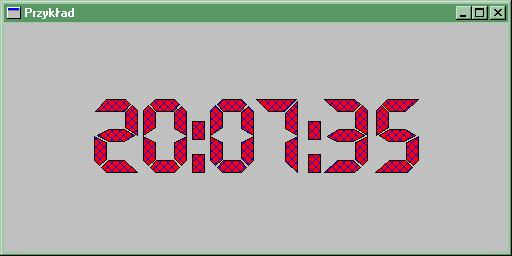
\includegraphics[width=0.75\textwidth]{./pic/p04}
\caption{Zegar elektroniczny, bardzo łatwo byłoby zrobić z niego budzik}
\end{center}
\end{figure}

\begin{scriptsize}
\begin{verbatim}
/*
 *
 * Zegar
 *
 */
#include <windows.h>

#define ID_TIMER    1

int xSize, ySize;

/* Deklaracje wyprzedzające */
LRESULT CALLBACK WindowProcedure(HWND, UINT, WPARAM, LPARAM);
void PaintCurrentTime( HDC hdc );

/* Nazwa klasy okna */
char szClassName[] = "PRZYKLAD";

int WINAPI WinMain(HINSTANCE hThisInstance, HINSTANCE hPrevInstance, 
                   LPSTR lpszArgument, int nFunsterStil)
{
    HWND hwnd;               /* Uchwyt okna */
    MSG messages;            /* Komunikaty okna */
    WNDCLASSEX wincl;        /* Struktura klasy okna */

    /* Klasa okna */
    wincl.hInstance     = hThisInstance;
    wincl.lpszClassName = szClassName;
    wincl.lpfnWndProc   = WindowProcedure;    // wskaźnik na funkcję obsługi okna  
    wincl.style         = CS_DBLCLKS;                 
    wincl.cbSize        = sizeof(WNDCLASSEX);

    /* Domyślna ikona i wskaźnik myszy */
    wincl.hIcon   = LoadIcon(NULL, IDI_APPLICATION);
    wincl.hIconSm = LoadIcon(NULL, IDI_APPLICATION);
    wincl.hCursor = LoadCursor(NULL, IDC_ARROW);
    wincl.lpszMenuName = NULL; 
    wincl.cbClsExtra = 0;   
    wincl.cbWndExtra = 0;   
    /* Jasnoszare tło */
    wincl.hbrBackground = (HBRUSH)GetStockObject(LTGRAY_BRUSH);

    /* Rejestruj klasę okna */
    if(!RegisterClassEx(&wincl)) return 0;

    /* Twórz okno */
    hwnd = CreateWindowEx(
           0,                   
           szClassName,         
           "Przykład",       
           WS_OVERLAPPEDWINDOW, 
           CW_USEDEFAULT,       
           CW_USEDEFAULT,       
           512,                 
           256,                 
           HWND_DESKTOP,        
           NULL,                
           hThisInstance,       
           NULL                 
           );

    ShowWindow(hwnd, nFunsterStil);
    /* Pętla obsługi komunikatów */
    while(GetMessage(&messages, NULL, 0, 0))
    {
           /* Tłumacz kody rozszerzone */
           TranslateMessage(&messages);
           /* Obsłuż komunikat */
           DispatchMessage(&messages);
    }

    /* Zwróć parametr podany w PostQuitMessage( ) */
    return messages.wParam;
}

/* Tę funkcję woła DispatchMessage( ) */
LRESULT CALLBACK WindowProcedure(HWND hwnd, UINT message, 
                                 WPARAM wParam, LPARAM lParam)
{
    PAINTSTRUCT ps; 
    RECT        r;
	HDC         hdc;

    switch (message)                  
    {
		   case WM_CREATE:
			   SetTimer(hwnd, ID_TIMER, 500, NULL);
			   break;
           case WM_TIMER:
               GetClientRect( hwnd, &r );
               InvalidateRect( hwnd, &r, 1 );
			   break; 
           case WM_PAINT:
               hdc = BeginPaint( hwnd, &ps );               
			   PaintCurrentTime( hdc );	
               EndPaint( hwnd, &ps );              
               break;
           case WM_SIZE:
			  xSize = LOWORD(lParam);
		      ySize = HIWORD(lParam);
			  break; 
           case WM_DESTROY:
              KillTimer(hwnd, ID_TIMER); 
              PostQuitMessage(0);        
              break;
           default:                   
              return DefWindowProc(hwnd, message, wParam, lParam);
    }
    return 0;
}

/* Maluj aktualny czas na ekranie */
void PaintCurrentTime( HDC hdc )
{
    char sTime[256];
    SYSTEMTIME time;
    HFONT      hFont;
    SIZE       size;
    
    // pobierz aktualny czas systemowy
    // i konwertuj go na zadany format
    GetSystemTime( &time );
    GetTimeFormat( LOCALE_SYSTEM_DEFAULT, 0, &time, 
                   "HH':'mm':'ss", sTime, 256 );

    // twórz font logiczny
	hFont = CreateFont( 112, 0, 0, 0, 
		                FW_NORMAL, 0, 0, 0, 
		                DEFAULT_CHARSET, OUT_DEFAULT_PRECIS,
		                CLIP_DEFAULT_PRECIS, DEFAULT_QUALITY,
		                DEFAULT_PITCH, "LED" );
	SelectObject( hdc, hFont );

    // licz rozmiar tekstu
    GetTextExtentPoint32 (hdc, sTime, lstrlen (sTime), &size) ;

    // rozpocznij ścieżkę graficzną
    BeginPath (hdc) ;

    SetBkMode( hdc, TRANSPARENT );
	TextOut( hdc, (xSize-size.cx)/2, (ySize-size.cy)/2, 
             sTime, strlen( sTime ) );               

    // zakończ ścieżkę
    EndPath (hdc) ;

    // rysuj ścieżkę odpowiednim pędzlem
    SelectObject (hdc, CreateHatchBrush (HS_DIAGCROSS, RGB (0, 0, 255))) ;
    SetBkColor (hdc, RGB (255, 0, 0)) ;
    SetBkMode (hdc, OPAQUE) ;
    StrokeAndFillPath (hdc) ;

    DeleteObject (SelectObject (hdc, GetStockObject (WHITE_BRUSH)));
    SelectObject (hdc, GetStockObject (SYSTEM_FONT)) ;
    DeleteObject (hFont) ;
}
\end{verbatim}
\end{scriptsize}

\subsection{Okna dialogowe}

Aplikacja złożona z jednego okna dialogowego jest oczywiście rzadkością. Zwykle zaprojektowanie
interfejsu użytkownika odpowiadającego modelowanemu problemowi wymaga od kilku do nawet kilkuset
róznych okien dialogowych. Programista tworzy nowe okno dialogowe za pomocą jednej z funkcji:

\begin{scriptsize}
\begin{verbatim}
int DialogBox(

    HINSTANCE hInstance,	// instancja aplikacji
    LPCTSTR lpTemplate,	// szablon okna
    HWND hWndParent,	// okno macierzyste
    DLGPROC lpDialogFunc 	// funkcja obsługi okna
   );	

HWND CreateDialog(

    HINSTANCE hInstance,	// instancja aplikacji
    LPCTSTR lpTemplate,	// szablon okna
    HWND hWndParent,	// okno macierzyste
    DLGPROC lpDialogFunc 	// funkcja obsługi okna
   );
\end{verbatim}
\end{scriptsize}

Funkcja DialogBox() tworzy tzw. {\em modalne} okno dialogowe, tzn. takie, które nie pozwala
użytkownikowi na uaktywnienie żadnego innego okna aplikacji do czasu zamknięcia okna dialogowego.
Funkcja CreateDialog() tworzy niemodalne okno dialogowe, tzn. okno z własną, niezależną pętlą obsługi 
komunikatów.

Obie z tych funkcji oczekują wskazania odpowiedniego szablonu okna. Szablon taki dodaje się do
zasobów aplikacji (zwykle ma rozszerzenie *.rc). Szablony okien dialogowych mają swoją specjalną składnię i
choć można wykonstruować okno bez dodawania szablonu do zasobów (szablon tworzy się dynamicznie, a następnie
korzysta się z funkcji CreateDialogIndirect() lub DialogBoxIndirect(), zaś okna potomne dodaje się 
przy obsłudze komunikatu WM\_INITDIALOG), to korzystanie z nich znacznie ułatwia cały proces.

\begin{scriptsize}
\begin{verbatim}
/* EX.C */
/*
 *
 * Okna dialogowe
 *
 */
#include <windows.h>

/* Deklaracja wyprzedzająca: funkcja obsługi okna */
LRESULT CALLBACK WindowProcedure(HWND, UINT, WPARAM, LPARAM);
BOOL DialogBoxWindowProcedure(HWND, UINT, WPARAM, LPARAM);
void CreateMyMenu( HWND hwnd );
/* Nazwa klasy okna */
char szClassName[] = "PRZYKLAD";

int WINAPI WinMain(HINSTANCE hThisInstance, HINSTANCE hPrevInstance, 
                   LPSTR lpszArgument, int nFunsterStil)
{
    HWND hwnd;               /* Uchwyt okna */
    MSG messages;            /* Komunikaty okna */
    WNDCLASSEX wincl;        /* Struktura klasy okna */

    /* Klasa okna */
    wincl.hInstance     = hThisInstance;
    wincl.lpszClassName = szClassName;
    wincl.lpfnWndProc   = WindowProcedure;    // wskaźnik na funkcję obsługi okna  
    wincl.style         = CS_DBLCLKS;                 
    wincl.cbSize        = sizeof(WNDCLASSEX);

    /* Domyślna ikona i wskaźnik myszy */
    wincl.hIcon   = LoadIcon(NULL, IDI_APPLICATION);
    wincl.hIconSm = LoadIcon(NULL, IDI_APPLICATION);
    wincl.hCursor = LoadCursor(NULL, IDC_ARROW);
    wincl.lpszMenuName = NULL; 
    wincl.cbClsExtra = 0;   
    wincl.cbWndExtra = 0;   
    /* Jasnoszare tło */
    wincl.hbrBackground = (HBRUSH)GetStockObject(LTGRAY_BRUSH);

    /* Rejestruj klasę okna */
    if(!RegisterClassEx(&wincl)) return 0;

    /* Twórz okno */
    hwnd = CreateWindowEx(
           0,                   
           szClassName,         
           "Przykład",       
           WS_OVERLAPPEDWINDOW, 
           CW_USEDEFAULT,       
           CW_USEDEFAULT,       
           512,                 
           512,                 
           HWND_DESKTOP,        
           NULL,                
           hThisInstance,       
           NULL                 
           );

    CreateMyMenu( hwnd );
    ShowWindow(hwnd, nFunsterStil);
    /* Pętla obsługi komunikatów */
    while(GetMessage(&messages, NULL, 0, 0))
    {
           /* Tłumacz kody rozszerzone */
           TranslateMessage(&messages);
           /* Obsłuż komunikat */
           DispatchMessage(&messages);
    }

    /* Zwróć parametr podany w PostQuitMessage( ) */
    return messages.wParam;
}

/* Tę funkcję woła DispatchMessage( ) */
LRESULT CALLBACK WindowProcedure(HWND hwnd, UINT message, 
                                 WPARAM wParam, LPARAM lParam)
{
    static HINSTANCE hInstance ;

    switch (message)                  
    {
           case WM_CREATE :
                hInstance = ((LPCREATESTRUCT) lParam)->hInstance ;
                break;  
           case WM_DESTROY:
                PostQuitMessage(0);        
                break;
           case WM_COMMAND:
                switch(LOWORD(wParam))
                {
                     case 100 : DialogBox( hInstance, MAKEINTRESOURCE(501), 
                                  hwnd, DialogBoxWindowProcedure ); break;
                     case 101 : SendMessage( hwnd, WM_CLOSE, 0, 0 );break;
                }   
           default:                   
              return DefWindowProc(hwnd, message, wParam, lParam);
    }
    return 0;
}

void CreateMyMenu( HWND hwnd )
{
	HMENU hMenu;
    HMENU hSubMenu;

	hMenu = CreateMenu () ;

	hSubMenu = CreateMenu () ;
	AppendMenu (hSubMenu, MF_STRING   , 100, "&Okno dialogowe") ;
	AppendMenu (hSubMenu, MF_SEPARATOR, 0  , NULL) ;
	AppendMenu (hSubMenu, MF_STRING   , 101, "&Koniec") ;
	AppendMenu (hMenu, MF_POPUP, (unsigned int)hSubMenu, "&Plik") ;

	SetMenu( hwnd, hMenu );
}

BOOL DialogBoxWindowProcedure(HWND hwnd, UINT message, 
                                 WPARAM wParam, LPARAM lParam)
{
    switch (message)                  
    {
           case WM_INITDIALOG:
              return TRUE ;
           case WM_COMMAND : 
              switch (LOWORD (wParam))
              {
                 case IDOK : case IDCANCEL :
                 EndDialog (hwnd, 0) ;
                 return TRUE ;
              }
    }
    return 0;
}

/* EX.RC */
#include <windows.h>

501 DIALOG 32, 32, 180, 40
STYLE WS_VISIBLE | WS_SYSMENU | WS_POPUP | WS_CAPTION | DS_MODALFRAME   
CAPTION "Okno dialogowe"
FONT 12,"Times New Roman"
BEGIN
   DEFPUSHBUTTON   "OK",IDOK,66,80,50,14
   CTEXT           "O programie...",-1,40,12,100,8
END
\end{verbatim}
\end{scriptsize}

Zauważmy, że funkcja obsługi komunikatów nie jest zwykłą funkcją obsługi komunikatów okna
Tak naprawdę obsługą komunikatów okna dialogowego zajmuje się domyślna funkcja obsługi komunikatów
okien dialogowych, istniejąca w systemie

\begin{scriptsize}
\begin{verbatim}
BOOL CALLBACK DialogProc(

    HWND hwndDlg,	// handle to dialog box
    UINT uMsg,	// message
    WPARAM wParam,	// first message parameter
    LPARAM lParam 	// second message parameter
   );	
\end{verbatim}
\end{scriptsize}

i to ona przekazuje komunikaty do funkcji obsługi komunikatów w oknie dialogowym.

Istnieją cztery zasadnicze różnice między zwykła funkcją obsługi okna, a funkcją obsługi okna dialogowego:
\begin{itemize}
\item zwykła funkcja obsługi okna zwraca wartość typu LRESULT, funkcja obsługi okna dialogowego zwraca BOOL
\item w przypadku nieobsługiwania jakiegoś komunikatu zwykła funkcja obsługi okna woła domyślną funkcję 
obsługi okien ({\em DefWindowProc}), zaś funkcja obsługi okna dialogowego zwraca wartość TRUE kiedy
obsługuje jakiś komunikat i FALSE jeśli go nie obsługuje
\item funkcja obsługi okna dialogowego nie musi obsługiwać komunikatów WM\_PAINT i WM\_DESTROY
\item funkcja obsługi okna dialogowego nie otrzymuje komunikatu WM\_CREATE, tylko WM\_INITDIALOG
\end{itemize}

Szablon okna dialogowego, oprócz opisu stylu okna i cech okien potomnych może zawierać m.in.
\begin{itemize}
\item wskazanie menu (MENU menu-name)
\item wskazanie czcionki (FONT font)
\item wskazanie klasy (CLASS "klasa")
\end{itemize}

Istnieje ponadto możliwość skorzystania z typowych okien dialogowych. Każde z tych
okien po zamknięciu zwraca zestaw parametrów niezbędnych do zidentyfikowania wyboru użytkownika.
\begin{itemize}

\item Okna do wyboru nazwy pliku
\begin{scriptsize}
\begin{verbatim}
BOOL GetOpenFileName(

    LPOPENFILENAME lpofn 	
   );

BOOL GetSaveFileName(

    LPOPENFILENAME lpofn 	
   );	
\end{verbatim}
\end{scriptsize}

\item Typowe okno wyboru koloru
\begin{scriptsize}
\begin{verbatim}
BOOL ChooseColor(

    LPCHOOSECOLOR lpcc 	
   );
\end{verbatim}
\end{scriptsize}

\item Typowe okno wyboru czcionki
\begin{scriptsize}
\begin{verbatim}
BOOL ChooseFont(

    LPCHOOSEFONT lpcf 	
   );
\end{verbatim}
\end{scriptsize}

\item Typowe okno ustalania parametrów drukowania
\begin{scriptsize}
\begin{verbatim}
BOOL PrintDlg(

    LPPRINTDLG lppd 	
   );	
\end{verbatim}
\end{scriptsize}

\end{itemize}

Przykład użycia okna do wyboru koloru:

\begin{scriptsize}
\begin{verbatim}
#include <windows.h>
#include <commdlg.h>
#include <stdio.h>

int WINAPI WinMain (HINSTANCE hInstance, HINSTANCE hPrevInstance,
                    PSTR szCmdLine, int iCmdShow)
{
     char buf[80];
     char *msgTpl = "Wybrano kolor o składowych: [%d, %d, %d]";

     static CHOOSECOLOR cc ;
     static COLORREF    crCustColors[16] ;

     cc.lStructSize    = sizeof (CHOOSECOLOR) ;
     cc.hwndOwner      = NULL ;
     cc.hInstance      = NULL ;
     cc.rgbResult      = RGB (0x80, 0x80, 0x80) ;
     cc.lpCustColors   = crCustColors ;
     cc.Flags          = CC_RGBINIT | CC_FULLOPEN ;
     cc.lCustData      = 0 ;
     cc.lpfnHook       = NULL ;
     cc.lpTemplateName = NULL ;

     if (ChooseColor (&cc))
     {
         sprintf( buf, msgTpl, 
                   GetRValue( cc.rgbResult ),
                   GetGValue( cc.rgbResult ),
                   GetBValue( cc.rgbResult ) );
         MessageBox( 0, buf, "", 0 );
     };
}
\end{verbatim}
\end{scriptsize}

\subsubsection{Powłoka systemu}
\label{powlokaSystemu}

Programista ma dostęp do powłoki systemu dzięki funkcji

\begin{scriptsize}
\begin{verbatim}
HINSTANCE ShellExecute(

    HWND hwnd,	// okno macierzyste
    LPCTSTR lpOperation,	// rodzaj operacji
    LPCTSTR lpFile,	// nazwa pliku
    LPCTSTR lpParameters,	// parametry
    LPCTSTR lpDirectory,	// domyślny katalog
    INT nShowCmd 	// flaga otwarcia okna
   );
\end{verbatim}
\end{scriptsize}

Powłoka potrafi wykonać na zadanym pliku kilka rodzajów operacji:
\begin{itemize}
\item "open"
\item "print"
\item "explore"
\item "properties"
\end{itemize}

